% -*- coding: UTF8 -*-
% \XeTeXinputencoding "UTF8"
\documentclass[a4paper,12pt]{examdesign}
\usepackage{tikz}
\usepackage{mathrsfs,pifont}
\usepackage{stmaryrd}
\usepackage{amsmath}
\usepackage[thinspace,thinqspace,squaren]{SIunits}
\usepackage[scale={.8,.8},footskip=12pt]{geometry}
\usepackage{lastpage,float}
\NumberOfVersions{1}
\usepackage[MnSymbol]{mathspec}
\usepackage[fullfamily,opticals,swash,minionint,openg,lf]{MinionPro}
\usepackage{xltxtra,xunicode}
\usepackage[PunctStyle=quanjiao]{xeCJK}
\setmainfont{Minion Pro}
\setmathfont(Greek){Minion Pro}
\setsansfont{Myriad Pro}
% \setmonofont{FreeMono}
\setCJKmainfont[BoldFont={FZSongHei-B07S},
              ItalicFont={FZKaiTi},
              SlantedFont={FZFangSongTi}]{FZShuSong-Z01}
\setCJKsansfont[BoldFont={FZDaHei-B02S},
              ItalicFont={FZLiShu II-S06S},
              SlantedFont={FZCuYuan-M03S}]{FZHeiTi}
\setCJKmonofont[BoldFont={FZZhongDengXian-Z07S},
              ItalicFont={FZXiYuan-M01S},
              SlantedFont={FZBaoSong-Z04S}]{FZXiDengXian-Z06S}
\usepackage{graphicx}
% \usepackage{floatflt}
\newcommand{\chuhao}{\fontsize{42pt}{\baselineskip}\selectfont}
\newcommand{\xiaochuhao}{\fontsize{36pt}{\baselineskip}\selectfont}
\newcommand{\yihao}{\fontsize{28pt}{\baselineskip}\selectfont}
\newcommand{\erhao}{\fontsize{21pt}{\baselineskip}\selectfont}
\newcommand{\xiaoerhao}{\fontsize{18pt}{\baselineskip}\selectfont}
\newcommand{\sanhao}{\fontsize{15.75pt}{\baselineskip}\selectfont}
\newcommand{\sihao}{\fontsize{14pt}{\baselineskip}\selectfont}
\newcommand{\xiaosihao}{\fontsize{12pt}{\baselineskip}\selectfont}
\newcommand{\wuhao}{\fontsize{10.5pt}{\baselineskip}\selectfont}
\newcommand{\xiaowuhao}{\fontsize{9pt}{\baselineskip}\selectfont}
\newcommand{\liuhao}{\fontsize{7.875pt}{\baselineskip}\selectfont}
\newcommand{\qihao}{\fontsize{5.25pt}{\baselineskip}\selectfont}

\def\Varangle#1{\kern.75pt\vtop{\hbox{\kern-.75pt$/{#1}$}\kern-.35pt\hrule}}

\begin{document}
\DeclareGraphicsExtensions{.pdf}
\renewcommand\figurename{图}
\newcommand\AnswerLeading{解}
\SectionPrefix{}
% \NoKey
\NoRearrange
\ShortKey
\ProportionalBlanks{1.5}
\SectionFont{\large\bf}
\examname{电子测量}
\DefineAnswerWrapper{\begin{description}\item [\AnswerLeading:]}{\end{description}}
\def\namedata{\large学号\underline{\hspace{126pt}}姓名\underline{\hspace{98pt}}成绩\underline{\hspace{98pt}}}
\class{\large学院(部)\underline{\hspace{98pt}}年级\underline{\hspace{98pt}}专业\underline{\hspace{98pt}}}
\begin{examtop}
\begin{center}
\begin{tabular}{r}
    {\Large \bf 苏州大学
    \underline{\hspace{54pt}\examtype\hspace{54pt}} 课程}\hspace{9pt}\medskip \\
    {\Large \bf 期 \underline{\hspace{9pt}末\hspace{9pt}} 试卷
    \hspace{9pt}(\Alph{version}) 卷\hspace{36pt}共 4 页}\medskip\\
    {\large考试形式 \underline{\hspace{7pt}闭卷\hspace{7pt}}\hspace{48pt}2015 年 1 月}
\end{tabular}
\\\bigskip
\classdata\\ \namedata
\end{center}
\bigskip
\end{examtop}
\begin{keytop}
\begin{center}
\begin{tabular}{r}
    {\Large \bf 苏州大学
    \underline{\hspace{54pt}\examtype\hspace{54pt}} 课程}\hspace{9pt}\medskip \\
    {\Large \bf \hspace{17pt}期 \underline{\hspace{6pt}末\hspace{6pt}}
    试卷 (\Alph{version}) 卷\hspace{9pt}参考答案\hspace{12pt}共 \pageref{LastPage} 页}\medskip\\
    {\large考试形式 \underline{\hspace{7pt}闭卷\hspace{7pt}}\hspace{48pt}2015 年 1 月}
\end{tabular}
\end{center}
\bigskip
\end{keytop}

\newcommand\mathdot[1]{\dot#1}

\begin{fillin}[title={一、填空题 (每题 2 分,共 20 分)}]
    \begin{question}
        示波器的水平通道主要由\blank{扫描发生器环}、触发电路和X放大器组成。
    \end{question}
    \begin{question}
        DVM的抗干扰能力可用\blank{串模干扰抑制比}和共模抑制比来表示。
    \end{question}
    \begin{question}
        \blank{计量}是为了保证量值的统一和准确一致的一种测量。
    \end{question}
    \begin{question}
        3 位数字欧姆表,测量某电阻读数为 \unit{1452}{\ohm}。当保留两位有效数字时,此电阻为\blank{1.5}kΩ。
    \end{question}
    \begin{question}
        电压测量仪器总的可分为两大类即模拟式的和\blank{数字}式的。
    \end{question}
    \begin{question}
        已知示波器的偏转灵敏度为
        $D_\mathrm{y}=\unit{0.5}{\volt}/\mathrm{div}$,荧光屏上显示波形
        的总高度为8格的两个周期的完整波形。则被测信号的峰峰值为
        \blank{\unit{4}{\volt}}。
    \end{question}
    \begin{question}
        引用相对误差又叫\blank{满度}相对误差。
    \end{question}
    \begin{question}
        所谓触发极性不是指触发信号本身的正负,而是指由它的\blank{上升}或下降沿触发。
    \end{question}
    \begin{question}
        峰值电压表的工作频率范围\blank{大}、输入阻抗高、灵敏度较高。
    \end{question}
    \begin{question}
        示波管由\blank{电子枪}、偏转系统、荧光屏三部分组成。
    \end{question}
\end{fillin}

\begin{shortanswer}[title={二、计算题 (每题 10 分,共 80 分)}]

\begin{question}
将下列数字保留 3 位有效数字进行舍入处理。
        \begin{equation*}
        \begin{aligned}
            73.449 &\Rightarrow  \\
            63.650 &\Rightarrow  \\
            832510 &\Rightarrow   \\
            0.007695 &\Rightarrow  
        \end{aligned}
        \end{equation*}
    \examvspace*{0cm}
    \begin{answer}
        \begin{equation*}
        \begin{aligned}
            73.449 &\Rightarrow 73.4 \\
            63.650 &\Rightarrow 63.6 \\
            832510 &\Rightarrow 8.33 \times 10^5 \\
            0.007695 &\Rightarrow 7.70 \times 10^{-3}
        \end{aligned}
        \end{equation*}
    \end{answer}
\end{question}
\begin{question}
    (1) 检定一只 2.5 级电流表 \unit{3}{mA} 量程的满度相对误差,手头有四
    块表,分别是:0.5 级 \unit{10}{mA} 量程;0.2 级 \unit{15}{mA} 量程;
    0.2 级 \unit{10}{mA} 量程;0.1 级 \unit{100}{mA} 量程。问哪块表最适
    合,为什么? \\
    (2) 1.5 级 \unit{100}{W} 量程的瓦特表,发现在 \unit{50}{W} 处的误
    差最大,为 \unit{1.4}{W},其它刻度的误差均小于 \unit{1.4}{W},问这块瓦特表是否合格?
    \examvspace*{5cm}
    \begin{answer}
        (1) 0.2 级 \unit{10}{mA} 量程表最合适误差最小。(2) 该表的最大引用误差为 $\gamma = 1.4\% < 1.5\%$,可见这块电压表合格。
    \end{answer}
\end{question}
\begin{question}
有一个信号源,对其输出电压 $U$ 进行 6 次测量(可认为是独立、等精密度,无
系统误差的测量),所得数据如下表:
\begin{table}[H]
\centering
\begin{tabular}{|r|c|c|c|c|c|c|}
    \hline
    序号 i &1 &2 &3 &4 &5 &6 \\ \hline
    电压 $U$ (V) &10.075 &10.085 &10.095 &10.065 &10.085 &10.080 \\
    \hline
\end{tabular}
\end{table}
(1) 计算平均值及其标准偏差估计值; \\
(2) 若要求置信概率 95\%,估计信号电压的真值约在什么范围内?
    \examvspace*{7cm}
    \begin{answer}
        (1) 求 $U$ 的平均值 $\overline{U} = \unit{1001.071}{V}$,由贝
        塞尔公式求 $U$ 的标准偏差估计值 $s(U) = \unit{0.871}{\volt}$,故
        平均值的标准偏差估计值为 $s(\overline{U}) = \unit{0.334}{\volt}$。
       (2) 由自由度及置信概率可从附录 II 查得相应的 $t_a = 2.571$。估计 $U$ 的
       真值所处区间:$1001.071 \pm 0.859 \unit{}{V}$,暨 [1000.212, 1001.930]\unit{}{V}。
    \end{answer}
\end{question}
\begin{question}
    用电子计数器测量一个 $f_x = \unit{100}{Hz}$ 的信号频率,采用测频 (选
    闸门时间为 \unit{1}{s}) 和测周 (选时标为 \unit{0.1}{\micro s}) 两种方法,试比较这两种方法的测量误差。
    \examvspace*{4cm}
    \begin{answer}
        测频时计数误差:$\frac{1}{T f_x} = 0.01$, 测周时计数误差:
        $\frac{1}{T_x f_c} = 1 \times 10^{-5}$
        所以在低频时测周的测量误差比测频的测量误差小。
    \end{answer}
\end{question}
\begin{question}
    设两个电阻 $R_1 = (150\pm0.6)\unit{}{\ohm}$,$R_2 =
    \unit{62}{\ohm}\pm 2\%$,试求此二电阻在串联及并联时的总阻值及其误差。
    \examvspace*{10cm}
    \begin{answer}
        $\Delta R_1=\unit{0.6}{\ohm}$,$\Delta R_2=62\times
        2\%=\unit{1.24}{\ohm}$。
        串联:$R= R_1+R_2=\unit{212}{\ohm}$。$\Delta R = \unit{1.84}{\ohm}$。
        $\gamma = 0.87\%$。
        并联:$R = \unit{43.9}{\ohm}$,$\Delta R = \unit{0.67}{\ohm}$,$\gamma
        = 1.53\%$。
    \end{answer}
\end{question}
\begin{question}
    在示波器上分别观察到峰值相等的正弦波、三角波和方波,
    $U_\mathrm{P}=\unit{10}{V}$,采取正弦波有效值刻度的电压表测量之,试求采用(1)峰值检波方式的读数,(2)均值检波方式的读数,(3)有效值检波方式的读数。
    \examvspace*{10cm}
    \begin{answer}
        (1) 峰值检波时三种波形读数均为 $\alpha =
        U_\mathrm{P}/k_\mathrm{P\sim} = \unit{7.07}{\volt}$。
        (2) 均值检波时读数 $\alpha = k_\mathrm{F\sim}\overline{U} =
        k_\mathrm{F\sim}U_\mathrm{P}/k_\mathrm{P}/k_\mathrm{F}$,三种
    波形平均值分别为 $6.37$、$5$、$10$,读数分别为 \unit{7.07}{V}、
    \unit{5.55}{V}、\unit{11.1}{V}。
       (3) 有效值检波 $\alpha = U_\mathrm{P}/k_\mathrm{P}$,读数分别为
       \unit{7.07}{V}、 \unit{5.77}{V}、\unit{10}{V}。
    \end{answer}
\end{question}
\begin{question}
    下图为一双环合成单元,其中内插振荡器的输出频率范围为 $\unit{30}{kHz}
    \sim\unit{40}{kHz}$,环 1 的分频比 N 变化范围为 $200\sim 500$,输入参考频率
    为 $\unit{10}{kHz}$,问该合成单元的输出频率范围是多少?
    \begin{figure}[H]
        \centering
        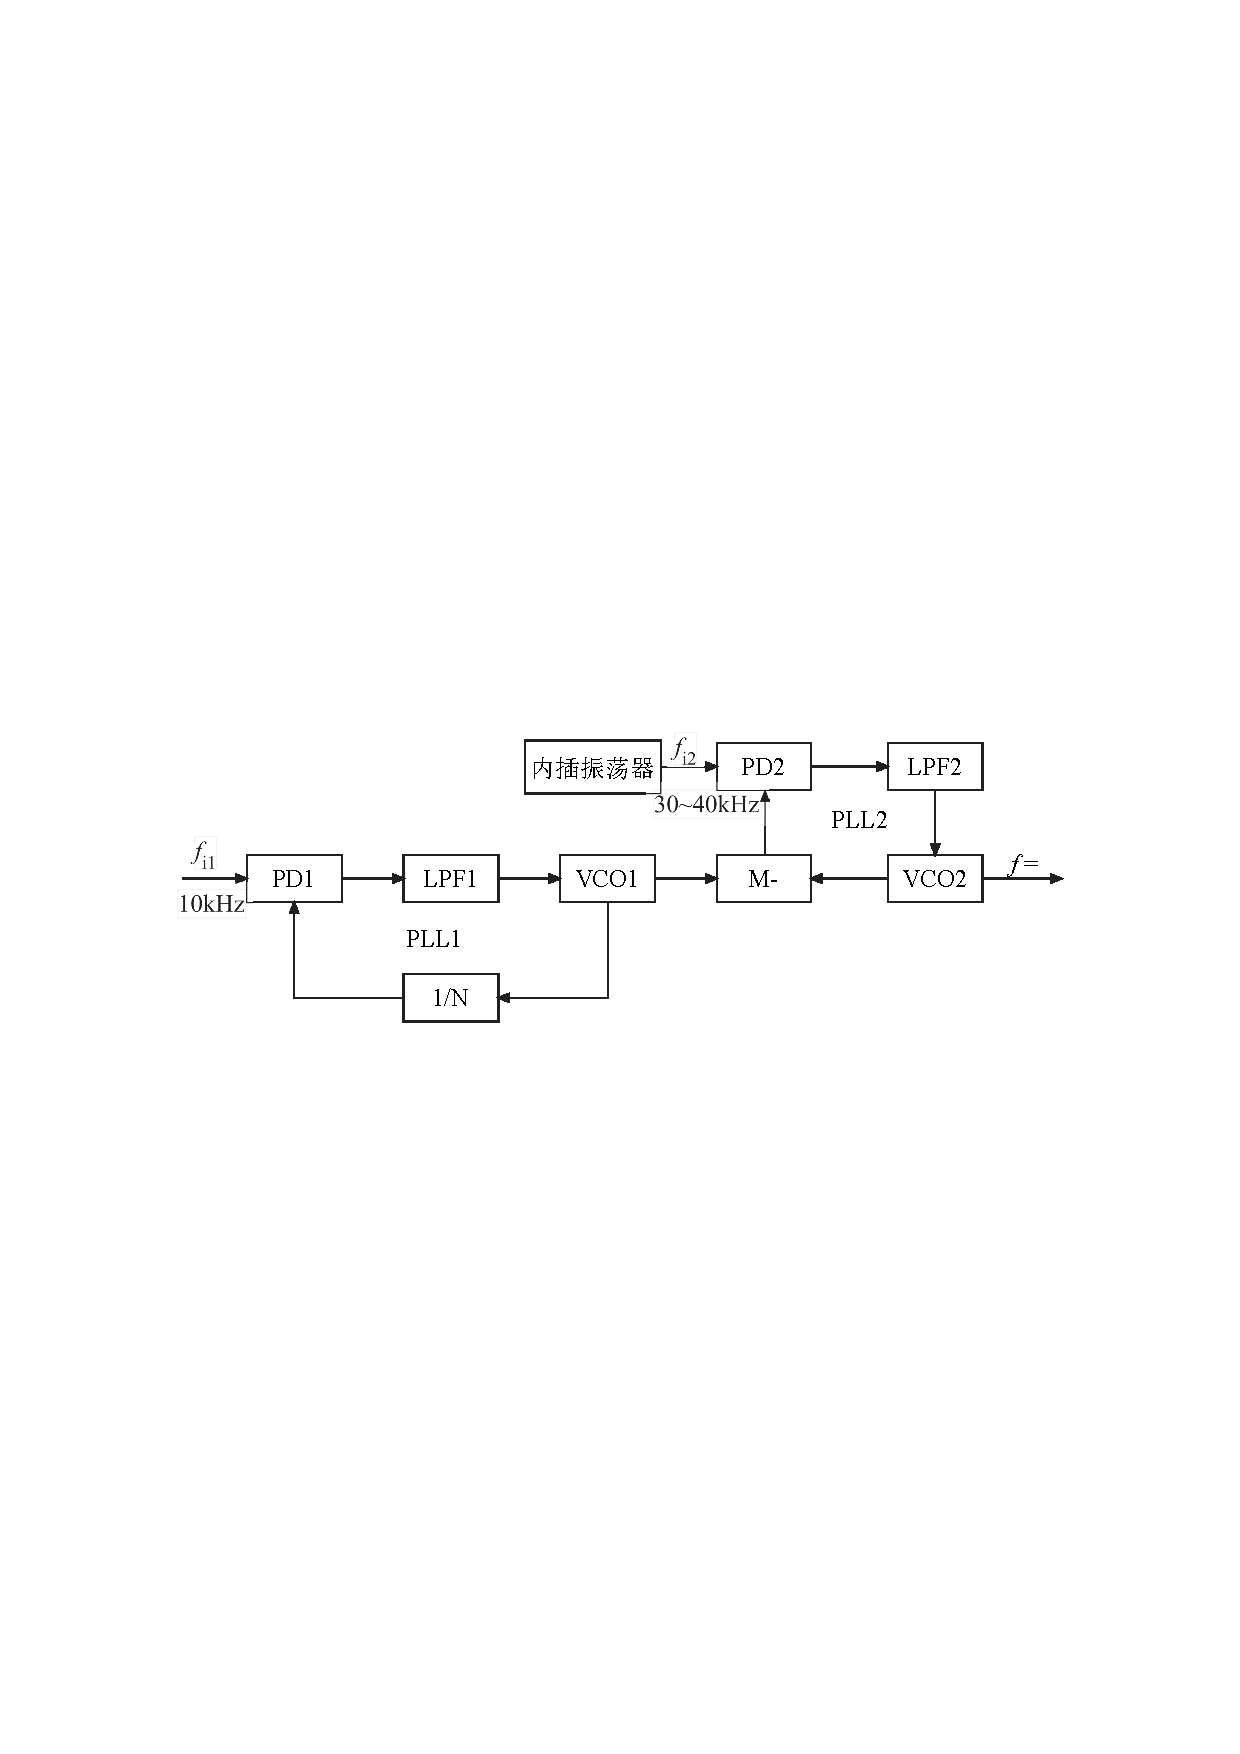
\includegraphics{pll}
    \end{figure}
    \examvspace*{4cm}
    \begin{answer}
        $f_o = N\times f_{i1}+f_{i2}$,所以 $f_o$ 范围为
        $2.030\sim\unit{5.040}{MHz}$。
    \end{answer}
\end{question}
\begin{question}
    已知示波器偏转灵敏度 $D_y=\unit{0.2}{V/cm}$,荧光屏有效宽度
    $\unit{10}{cm}$。 \\
    (1) 若扫描速度为 $\unit{0.05}{ms/cm}$ (放“校正”位置),观察到正弦波两个周期
    正好在水平方向占 $\unit{10}{cm}$,垂直方向正好占据 $\unit{6}{cm}$。
    求被测信号的峰-峰值及频率。 \\
    (2) 若想在屏上显示 10 个周期的波形,扫描速度应取多大?
    \examvspace*{0cm}
    \begin{answer}
        (1) $U_\mathrm{PP} = 6 \times 0.2 = \unit{1.2}{\volt}$,$T = 5
        \times 0.05 = \unit{0.25}{ms}$,$f=1/T=\unit{4}{kHz}$。
        (2) $S_\mathrm{S} = 10 \times 0.25 / 10 = \unit{0.25}{ms/cm}$。
    \end{answer}
\end{question}

\end{shortanswer}
\end{document}
